\documentclass[10pt,conference]{IEEEtran}
\IEEEoverridecommandlockouts
\usepackage{cite}
\usepackage[utf8]{inputenc}
\usepackage[T1]{fontenc}
\usepackage[UTF8]{ctex}
\usepackage{amsmath,amssymb,amsfonts}
\usepackage{algorithmic}
\usepackage{graphicx}
\usepackage{textcomp}
\usepackage{xcolor}
\usepackage{enumitem}
\usepackage{multirow}
\usepackage{tabularx}
\usepackage{array}
\usepackage{booktabs}
\usepackage{siunitx}
\usepackage{adjustbox}

\def\BibTeX{{\rm B\kern-.05em{\sc i\kern-.025em b}\kern-.08em
    T\kern-.1667em\lower.7ex\hbox{E}\kern-.125emX}}
\begin{document}

\title{面向 RISC\,-V 构建失败根因分析的\\日志压缩与规则学习方法%
\thanks{本工作得到中国科学院软件研究所等相关项目的支持。}}

\author{%
\IEEEauthorblockN{王泽华}
\IEEEauthorblockA{中国科学院软件研究所\\
中国科学院大学}}

\maketitle

\begin{abstract}
近年来，RISC\,-V 依托开源、模块化与可扩展等特性，正在成为新一代通用与专用处理器的重要架构选择。大量开源软件包被迁移到 RISC\,-V 平台，同时也暴露出构建失败高发、原因复杂且随上游演进不断反复的问题。构建日志往往规模巨大、结构异构且噪声众多，真正决定失败的关键线索常被淹没在不同阶段、相距甚远的输出片段中，传统基于人工经验或规则匹配的排查方式效率低、成本高，难以支撑大规模迁移实践。

本文面向 RISC\,-V 软件包构建失败场景，提出一套"日志压缩 + 规则学习"的根因分析方法。首先，设计面向长程因果依赖的多粒度语义日志压缩流程（MGSC），通过显式错误锚点定位、基于实体的跨距离上下文回溯以及轻量语义压缩模型，在严格 \emph{token} 预算下高保真保留与根因相关的关键信息。随后，提出基于历史修复经验的规则学习与根因推理方法（HRL-RCA），从历史修复记录中抽取结构化修复规则，构建按错误类型与构建阶段组织的规则树索引，结合压缩日志摘要进行条件匹配与推理，输出可解释的根因分类与修复建议。

基于来自实际 OBS 生产环境的 RISC\,-V 构建失败数据集的实验结果表明，所提出方法在关键错误行覆盖率、根因识别准确率以及修复建议质量等方面均优于多种基线方法，同时在日志压缩率和推理开销上保持良好平衡。
\end{abstract}

\begin{IEEEkeywords}
RISC\,-V，构建失败，根因分析，日志压缩，大语言模型
\end{IEEEkeywords}

%% ===== 第一章 绪论 =====
\section{绪论}

近年来，RISC\,-V 依托开源、模块化与可扩展等特性快速发展\cite{r1,r4}，逐渐成为新一代通用计算与专用计算的重要选择方向之一。随着产业界与学术界对 RISC\,-V 的持续投入，大量主流开源软件正在向 RISC\,-V 架构迁移\cite{r16}。然而由于主流开源软件的上游长期以 x86 和 ARM 为核心支持对象，其持续版本迭代往往不断引入新的架构强绑定特性，导致大量原本已适配 RISC\,-V 的软件包在跟随上游更新后再次构建失败。如图~\ref{fig:migration-trend} 所示，RISC\,-V 开源软件迁移的目标包数量与构建失败绝对数量均呈持续增长态势，加上数千个难以移植的长尾软件，RISC\,-V 生态建设本质上是一个高度动态且工作量持续增长的长期工程。

\begin{figure}[htbp]
    \centering
    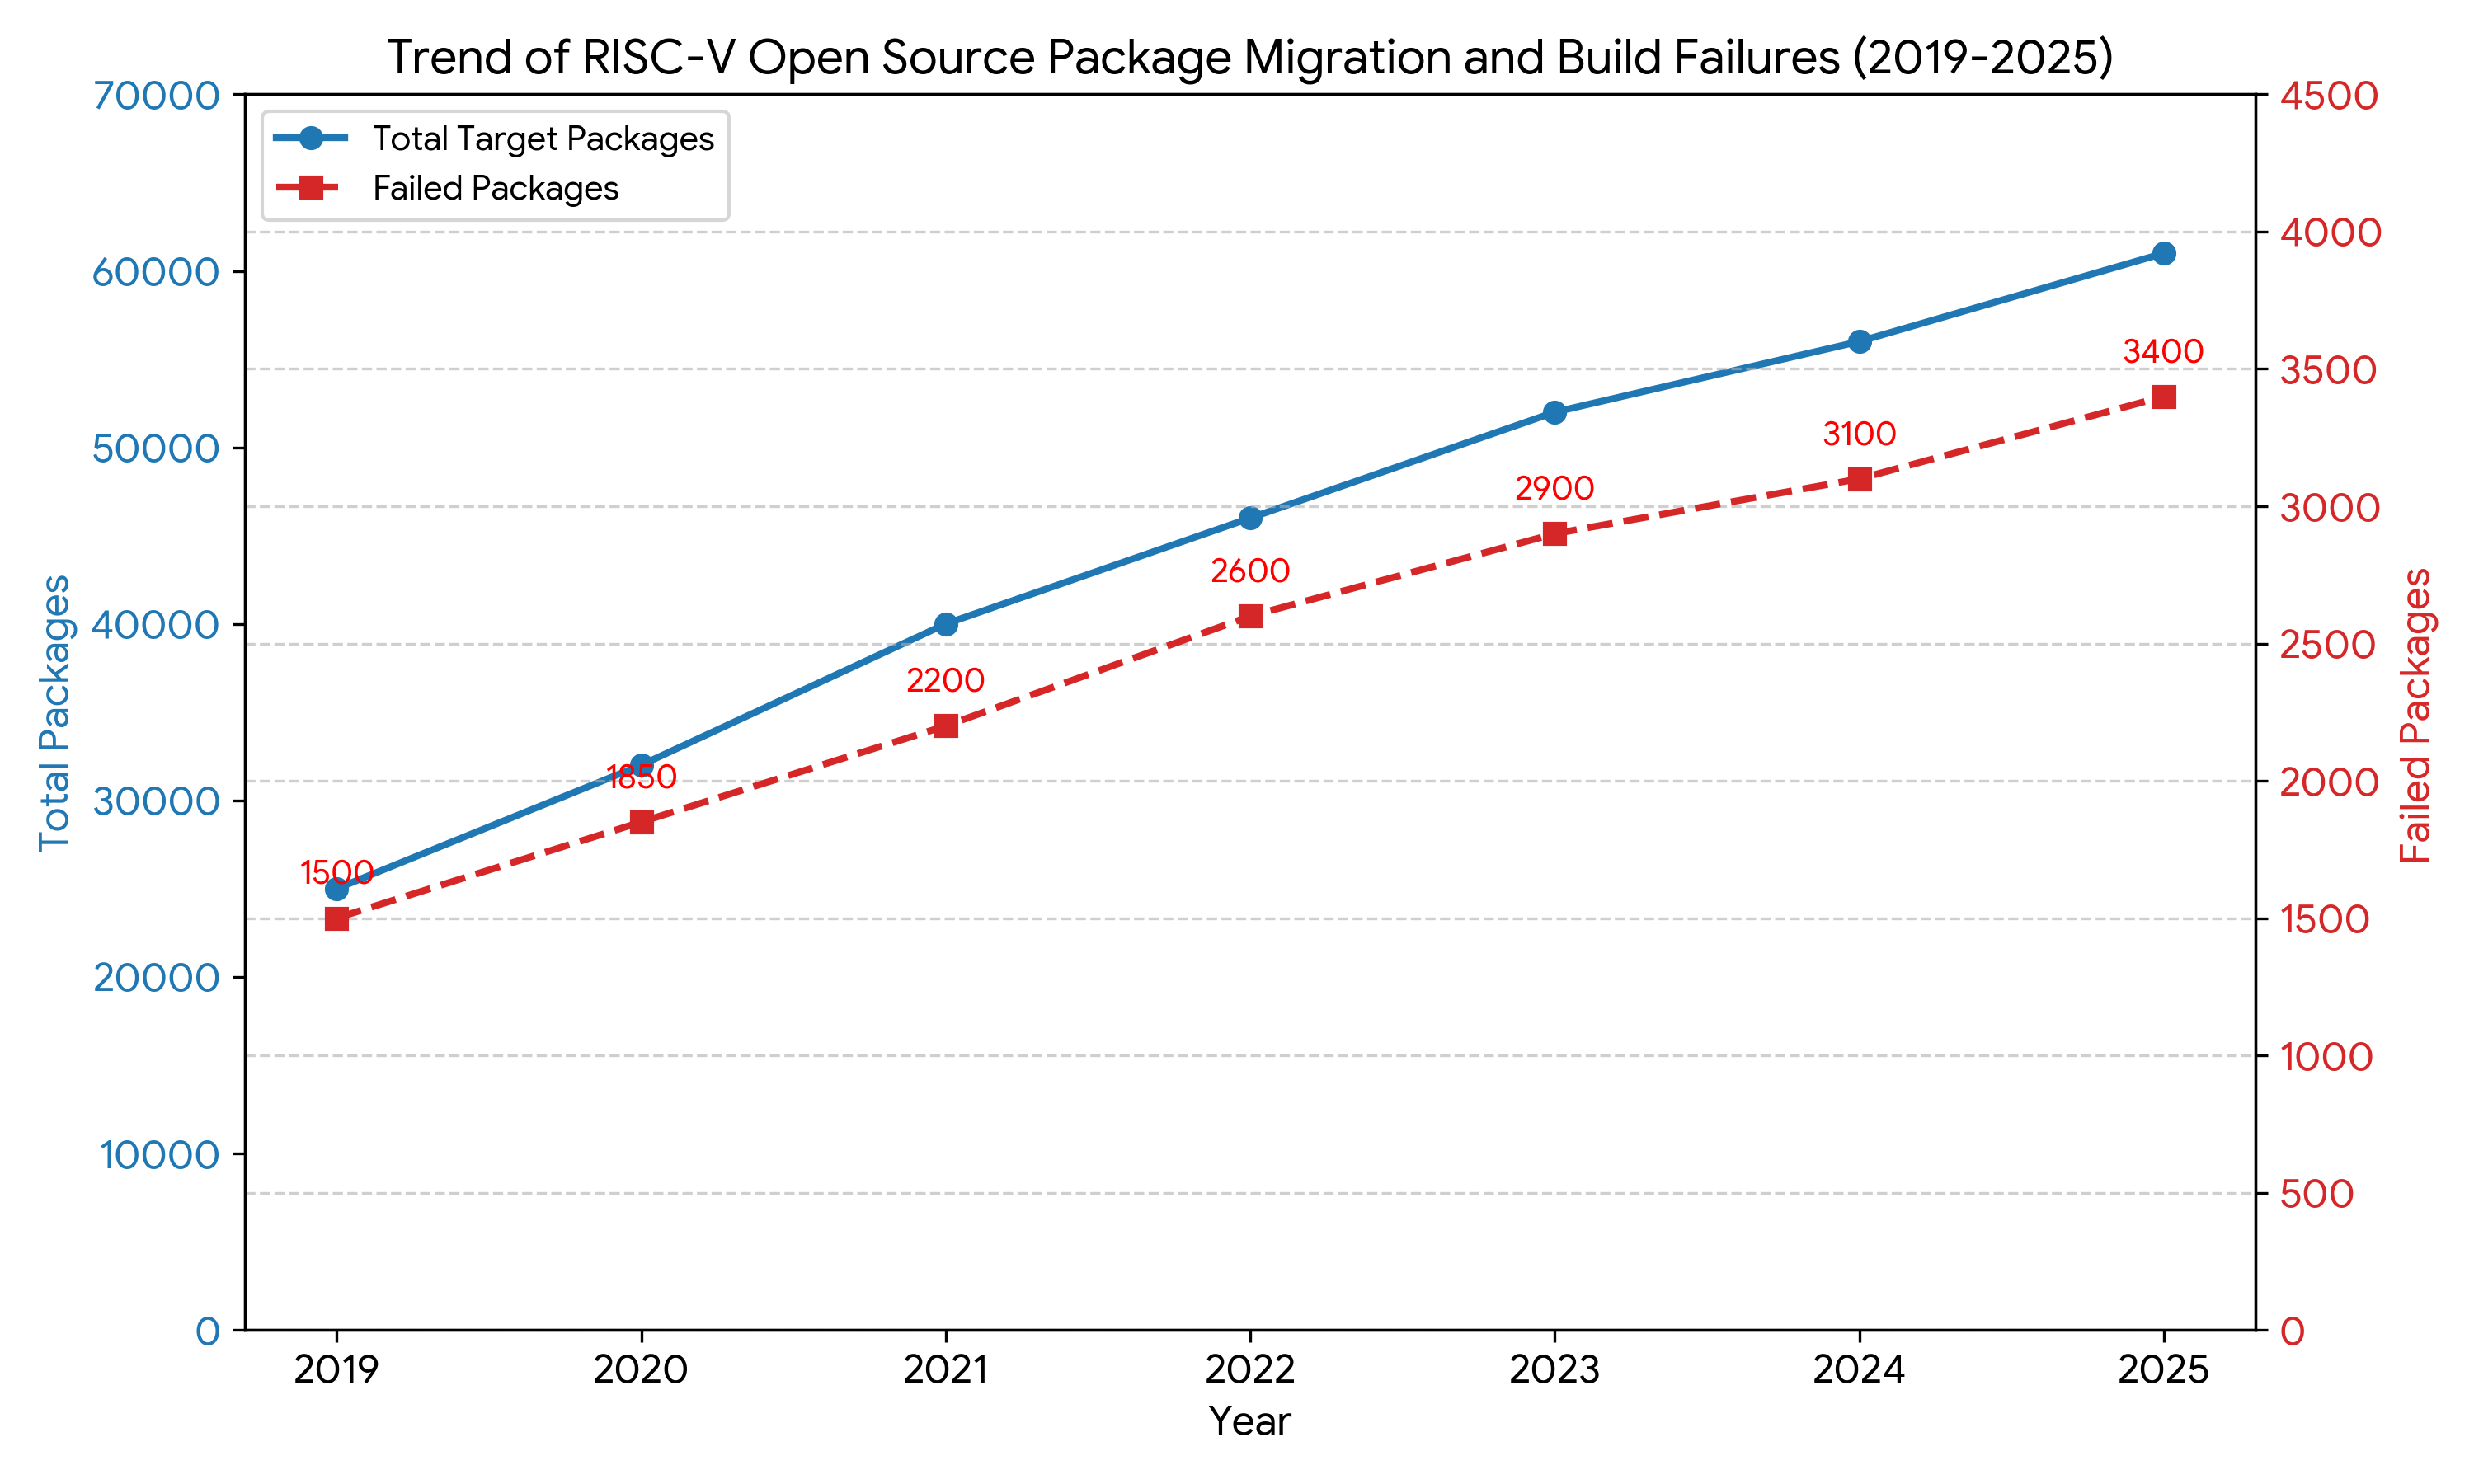
\includegraphics[width=1\linewidth]{pic/migration-trend.png}
    \caption{RISC\,-V 开源软件包迁移与构建失败趋势}
    \label{fig:migration-trend}
\end{figure}

在发行版级的软件包迁移实践中，开放构建服务（OBS）等平台通过自动化的构建、依赖管理与发布流程，为跨发行版、跨架构的软件包构建提供了统一基础设施。然而在 OBS 这类高度自动化的流水线中，构建失败呈现更高的频发性与多样性：同一软件包在不同架构、不同依赖版本、不同构建阶段（如~\texttt{\%prep}、\texttt{\%build}、\texttt{\%install}、\texttt{\%check}）均可能触发错误，且错误往往由架构差异、依赖链约束、构建脚本配置与补丁变更等多因素共同作用\cite{r12,r13}。构建日志通常规模巨大（数万至数十万行），真正与失败相关的关键信息不足 5\%，且日志格式在不同软件包与构建阶段间差异极大。更重要的是，很多时候最后出现的报错只是结果，真正触发失败的原因可能早在更前面的阶段就已出现，形成长程因果依赖。

\begin{table}[htbp]
\centering
\caption{不同排查方法对比}
\label{tab:method-compare}
\begin{tabularx}{\columnwidth}{|l|X|X|}
\hline
\textbf{方法} & \textbf{优势} & \textbf{局限性} \\
\hline
人工排查 & 准确率高，能处理复杂跨层依赖 & 依赖专家经验，效率低、成本高 \\
\hline
传统日志分析 & 速度快，适合格式稳定的日志 & 对异构日志泛化差，难以生成修复动作 \\
\hline
直接应用大模型 & 语义理解能力强，无需繁复规则 & 受限 token 预算，易产生幻觉 \\
\hline
\end{tabularx}
\end{table}

如表~\ref{tab:method-compare} 所示，现有方案难以同时兼顾处理长日志的效率、跨层级归因的准确性以及修复建议的可验证性。面向 RISC\,-V 软件包迁移的构建失败分析，亟需一种能够在有限 token 上下文预算下保留高保真证据链、并将历史修复经验以可判定条件与可追溯证据的方式组织起来的自动化方法。

本文的核心挑战有二。\textbf{挑战一}：如何从超长日志中找准真正的错误——关键报错被大量噪声淹没，真正触发失败的原因可能早在数百行前出现，仅截取报错附近的窗口容易错过因果线索。\textbf{挑战二}：如何从历史案例中找对能用的修复参考——修复经验分散在不同仓库的提交记录与 issue 讨论中，相似日志并不等价于适用修复，版本/依赖/阶段不同时可能产生误导。

针对上述挑战，本文做出以下贡献：
\begin{enumerate}
\item 提出面向长程因果依赖的多粒度语义日志压缩方法（MGSC），通过"显式错误锚点定位—基于实体的跨距离上下文回溯—轻量模型细粒度语义压缩"三阶段流水线，在严格 token 预算下高保真保留关键证据链。
\item 提出基于历史修复经验的规则学习与根因推理方法（HRL-RCA），将修复经验抽取为结构化规则并按"错误类型—构建阶段—适用前提"组织为树形索引，在线推理时通过条件路由召回满足前提的规则，结合 ReAct 范式生成可追溯的根因分析与修复建议。
\item 基于 OBS 生产环境构建 RISC\,-V 构建失败数据集并开展系统实验，结果表明 MGSC 在关键证据覆盖率上优于现有压缩方法，HRL-RCA 在综合诊断得分上达到 79.0\%，显著超过多种基线，同时处理耗时降低约 61\%。
\end{enumerate}


%% ===== 第二章 相关工作 =====
\section{相关工作}

\subsection{日志解析与语义压缩}

日志解析旨在将非结构化日志归一化为事件模板与动态参数的结构化表示。早期方法依赖规则与正则匹配，典型如 SLCT\cite{r18} 通过聚类算法挖掘日志模式、Drain\cite{r20} 通过固定深度解析树实现在线高效解析，Logram\cite{r17} 利用 $n$-gram 字典加速模板识别。随着深度学习的发展，基于 LSTM 的方法\cite{r5} 学习正常执行路径的时序规律以检测异常；基于 Transformer 与自监督学习的方法获得更强的语义表征能力\cite{r6}。然而这些方法在跨系统、跨版本迁移时面临泛化不足的问题。

近年来，大语言模型（LLM）为日志解析提供了新的范式\cite{r8}。基于 prompt 的少样本日志解析\cite{r21}通过示例选择降低调用成本；DivLog\cite{r22} 通过上下文学习提升跨域解析能力；面向可解释性的在线日志分析方法\cite{r10}通过提示策略增强 LLM 的日志理解能力。面向 CI/CD 场景的日志分析框架\cite{r9}提出 token 高效的预处理与结构化诊断流程。然而在软件包构建失败这类长程因果依赖强、阶段跨度大的场景中，如何在有限 token 预算下稳定保留可追溯证据链，仍需更贴合任务特性的压缩方法。

\subsection{基于日志的根因分析}

根因分析（RCA）旨在从系统输出中定位故障的底层原因。传统方法通过规则关联完成事件匹配\cite{r19}，或结合源码分析推断失败执行路径\cite{r14}。深度学习方法将根因分析表述为日志行相关性排序任务，从日志中抽取故障指示性描述与参数用于结构化诊断\cite{r12}。

LLM 驱动的 RCA 更强调直接从故障日志出发生成可读的诊断结论。RCAgent\cite{wang2024rcagent} 通过工具增强的 LLM 智能体实现自主诊断，基于 Agent 的设计让模型通过多步推理逐步缩小根因范围。基于检索增强的方法\cite{r13}将多源信息组织为 LLM 可消费的上下文完成排障建议。然而，仅依赖"相似日志检索 + 自由生成"容易引入误导证据或放大幻觉，必须把适用前提、证据对齐与验证机制纳入体系化方案。本文方法正是从历史修复经验中学习可判定规则，并以树形索引实现条件路由，从源头降低误导风险。


%% ===== 第三章 方法 =====
\section{方法}

本文采用两阶段流水线处理 RISC\,-V 构建失败。第一阶段（MGSC）对超长日志进行多粒度语义压缩，输出以关键错误行为中心、包含必要上下文的结构化摘要。第二阶段（HRL-RCA）以压缩摘要为输入，结合历史修复经验的规则树索引，通过条件路由与 ReAct 推理生成可追溯的根因分析与修复建议。

\subsection{MGSC：多粒度语义日志压缩}\label{sec:mgsc}

构建失败日志的压缩并非简单删掉大部分行，而是要在有限预算内尽可能保留能支撑根因分析的关键证据。MGSC 以显式错误信息为锚点快速定位失败表征，再以关键实体为线索跨距离回溯补齐触发条件，最后在候选证据集上进行细粒度语义压缩与结构化整理。

\begin{figure*}
    \centering
    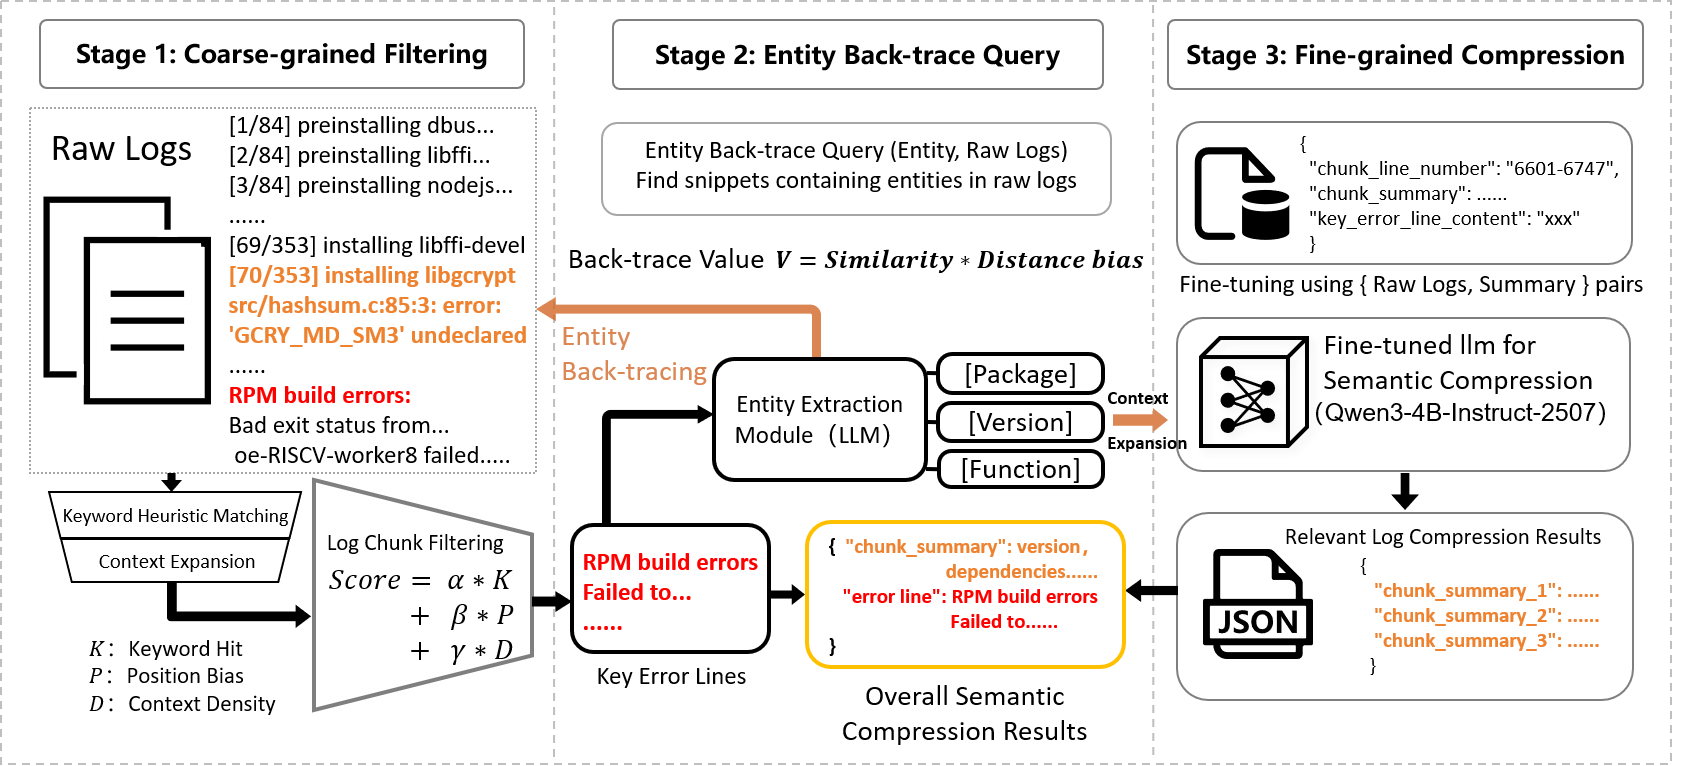
\includegraphics[width=1\linewidth]{pic/mgsc-overview.png}
    \caption{MGSC 多粒度语义日志压缩方法整体流程}
    \label{fig:mgsc}
\end{figure*}

如图~\ref{fig:mgsc} 所示，MGSC 分为三个阶段：

\subsubsection{快速粗粒度过滤}
首先通过正则规则集合 $R_{drop}$ 去除跨包稳定出现但与失败无关的冗余输出（如编译器版本回显、下载进度、固定格式状态提示等），得到过滤后日志 $L' = \{l_i \in L \mid g(l_i) = 1\}$。随后通过分层关键词匹配（强错误模式如 \texttt{error:}、\texttt{fatal}，构建终止提示如 \texttt{RPM build errors}，补充召回模式如 \texttt{undefined symbol}）召回关键错误行集合 $A$，并对重复报错进行去重聚合。

对每条关键错误行做前后窗口扩展生成候选日志块 $\mathcal{B}$，并按以下行级评分函数衡量重要性：
\begin{equation}
S(l_i) = \alpha \cdot I_{key}(l_i) + \beta \cdot f_{pos}(i) + \gamma \cdot D_{context}(i)
\end{equation}
其中 $I_{key}$ 为关键词匹配指示函数，$f_{pos}(i) = e^{-\lambda(N-i)/N}$ 为位置偏置项（越靠近日志末尾权重越高），$D_{context}$ 为局部关键词密度项。块级得分取块内行得分的聚合值，在 token 预算约束下选择 Top-n 块输出。

\subsubsection{基于实体的上下文回溯}
粗粒度过滤仅保留错误附近片段，难以覆盖跨阶段的触发线索（如更早的依赖探测失败）。本阶段从关键错误行中抽取实体线索（如缺失的库名、未定义符号、关键路径、编译选项等），以实体为查询条件在原始日志中检索相关片段。对每行 $l_j$ 定义回溯价值：
\begin{equation}
V(l_j) = \max_{e \in E}\left(\mathrm{Sim}(l_j, e) \cdot \frac{1}{\log(1 + \lambda \Delta t(l_j, e))}\right)
\end{equation}
其中 $\mathrm{Sim}$ 表示模糊匹配相似度，距离项保证在相似度相当时偏向更近的行。系统选取高价值命中行并聚合为回溯片段，补全长程因果链。

\subsubsection{细粒度语义压缩}
回溯得到的片段仍可能冗余偏长，本阶段使用领域微调的轻量模型（基于 Qwen3-4B-Instruct 微调）对回溯片段进行面向根因分析的摘要凝练。微调训练集包含 2925 条高质量日志块语义压缩数据，采用 SFT + LoRA 参数高效微调。实验表明，微调后模型的压缩比由 19.66$\times$ 提升至 30.6$\times$，同时关键错误覆盖率从 74.3\% 提升至 75.7\%。最终将细粒度摘要与粗粒度阶段的显式错误信息融合，输出结构化压缩结果 $S$。


\subsection{HRL-RCA：基于历史修复经验的规则学习与根因推理}\label{sec:hrl}

\begin{figure*}
    \centering
    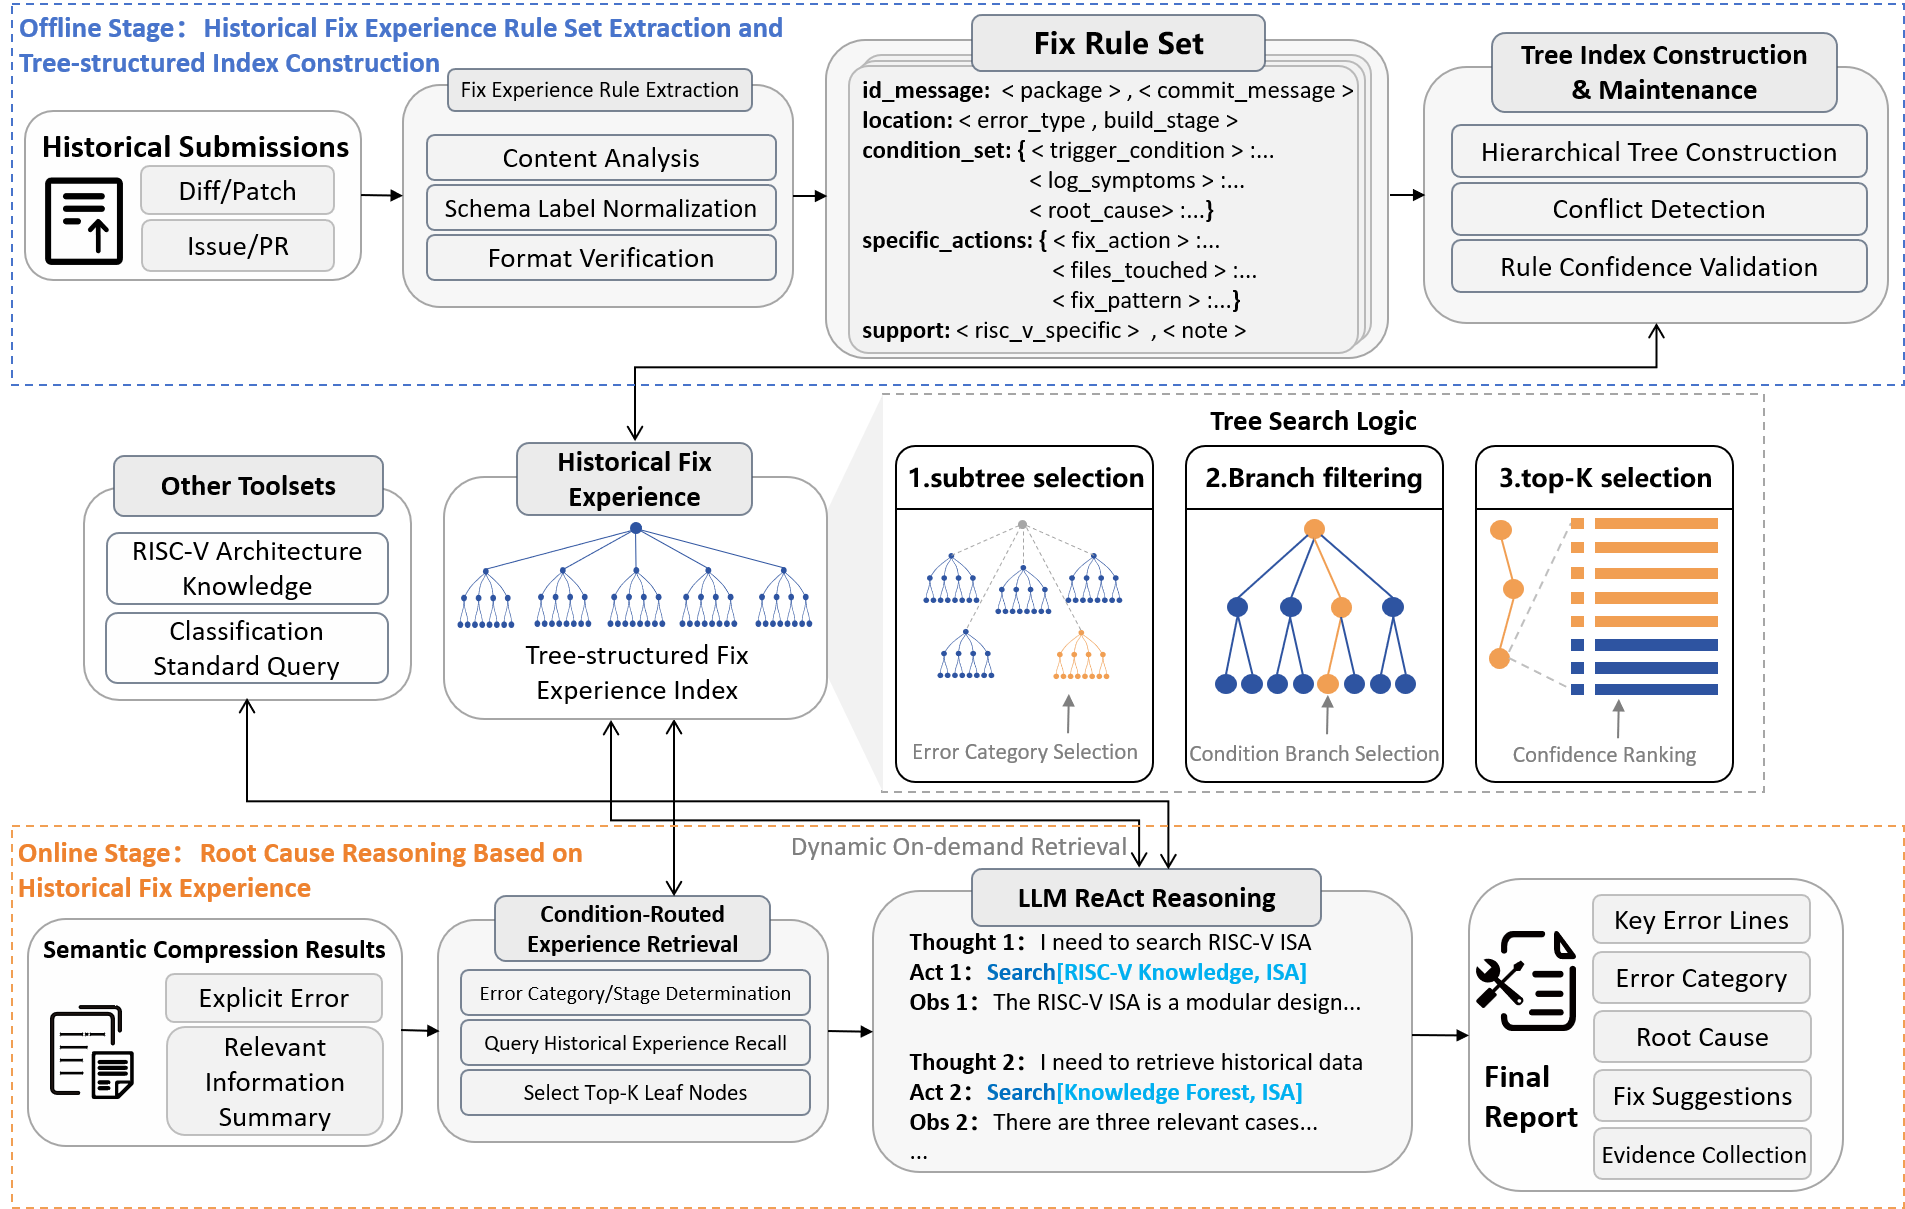
\includegraphics[width=1\linewidth]{pic/hrl-rca-overview.png}
    \caption{HRL-RCA 基于历史修复经验的规则学习与根因推理框架}
    \label{fig:hrl-overview}
\end{figure*}

如图~\ref{fig:hrl-overview} 所示，HRL-RCA 分为离线构建与在线推理两部分。离线阶段从历史提交记录中抽取修复规则并构建树形索引；在线阶段以 MGSC 输出的压缩摘要为入口，沿索引进行条件路由并在证据约束下生成诊断报告。

\subsubsection{历史修复信息结构化}
以单条修复提交为对象，输入包含 commit message、diff/patch、spec 变更及关联 issue/PR 讨论，输出为结构化 JSON 记录，字段包括：错误大类（error\_type）、构建阶段（build\_stage）、触发条件（trigger\_condition）、日志症状（log\_symptoms）、根因解释（root\_cause）、修复动作（fix\_action）、变更文件（files\_touched）等。构建流程采用"传统解析预处理—大模型结构化—校验与规范化"三级流水线，保证进入知识库的规则具有稳定格式与可追溯证据。

\subsubsection{修复规则树形索引构建与维护}
借鉴人工排障"先判别错误类别与阶段，再依据前提缩小范围"的逻辑，本方法将修复规则按"错误大类—构建阶段—可判定条件"组织为树形索引。如图~\ref{fig:rule-tree} 所示，第一层按五个问题域划分（架构兼容、版本兼容、依赖配置、编译配置、其他错误），第二层按构建阶段组织，更深层由触发条件驱动分叉，叶节点挂载具体修复规则集合并绑定 fix\_action 与适用前提。

\begin{figure}[htbp]
    \centering
    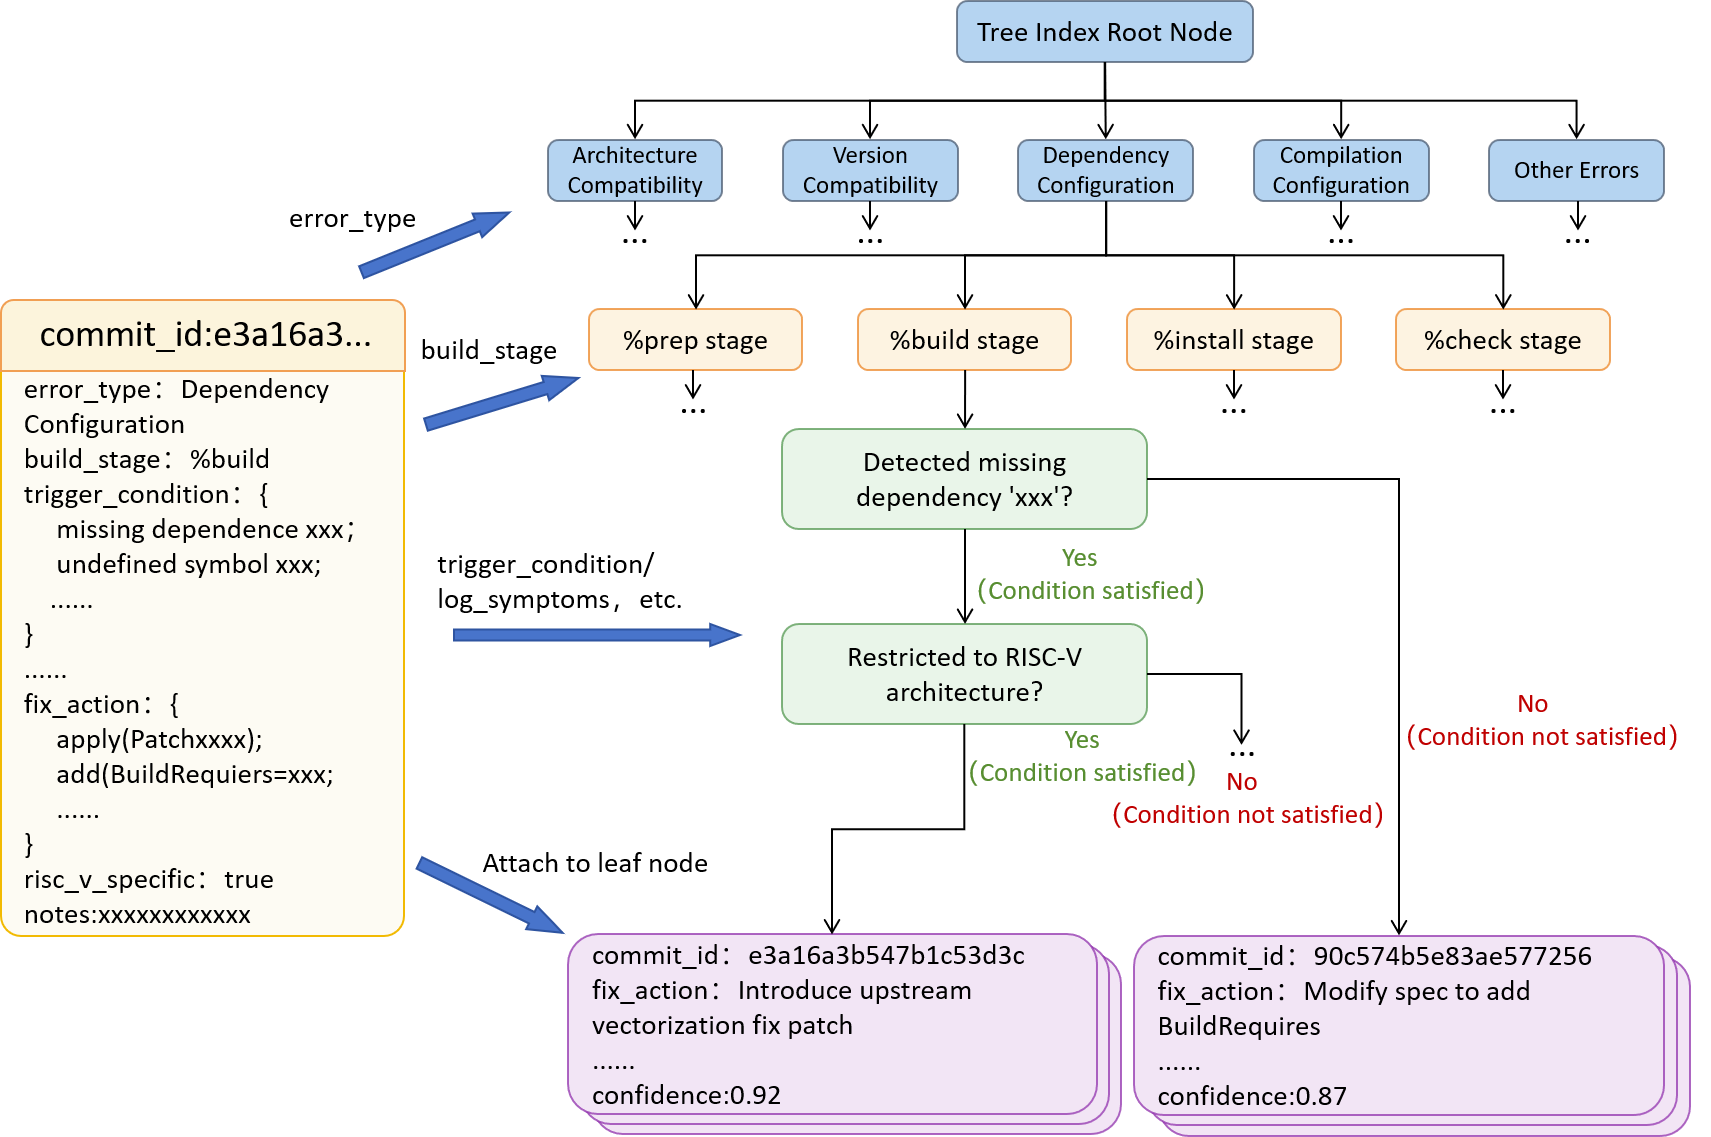
\includegraphics[width=1\linewidth]{pic/rule-tree.png}
    \caption{修复规则树形索引结构示意}
    \label{fig:rule-tree}
\end{figure}

为支持持续演进，设计增量更新与冲突检测合并机制。当新规则的条件集合与已有规则存在包含关系时，通过细化或泛化调整树结构。同时引入规则置信度进行质量控制：
\begin{equation}
\mathrm{Conf}(r) = \alpha \cdot S_{evi}(r) + (1-\alpha) \cdot S_{time}(r)
\end{equation}
其中 $S_{evi}(r) = n_r / (n_r + k)$ 为证据支持度（$n_r$ 为支撑记录数，$k$ 为平滑常数），$S_{time}(r) = 1 / (1 + (t_{now} - t_r)/T)$ 为时间新鲜度。低于阈值的规则进入待审核状态。

\subsubsection{在线根因推理}
在线阶段以 MGSC 输出的压缩摘要 $S$ 为入口：首先完成错误类型与构建阶段判定以定位索引入口节点；随后沿条件分支进行匹配，召回候选叶节点中的修复规则并按匹配度与置信度排序；最后采用 ReAct 范式将"摘要证据 + 路由路径 + 修复规则"注入上下文，要求模型以结构化格式输出根因解释与修复方案，并显式给出适用前提与证据引用。若检索到多条候选经验，系统输出主推荐与备选方案，并说明各自的适用边界。


%% ===== 第四章 实验评估 =====
\section{实验评估}

\subsection{实验设置}

\subsubsection{数据集}
实验数据来自 OBS 真实生产环境下的 RISC\,-V 软件包构建失败日志。日志压缩实验使用 133 个不同软件包的构建日志，总计 149219 行日志文本，并由专家标注 4582 行关键修复相关日志行作为评测基准。根因分析实验使用 174 个典型构建失败案例，覆盖五种错误类型（架构兼容、编译配置、依赖配置、版本兼容、其他错误）。

如图~\ref{fig:dataset} 所示，数据集中版本兼容类错误占比最高（29.9\%），编译配置与依赖配置各占 23.6\%，其他错误 14.4\%，架构兼容 8.6\%。从构建阶段分布看，\texttt{\%build} 阶段占 50.0\%，\texttt{\%prep} 占 24.1\%，\texttt{\%check} 占 20.7\%，\texttt{\%install} 占 5.2\%。

\begin{figure}[htbp]
    \centering
    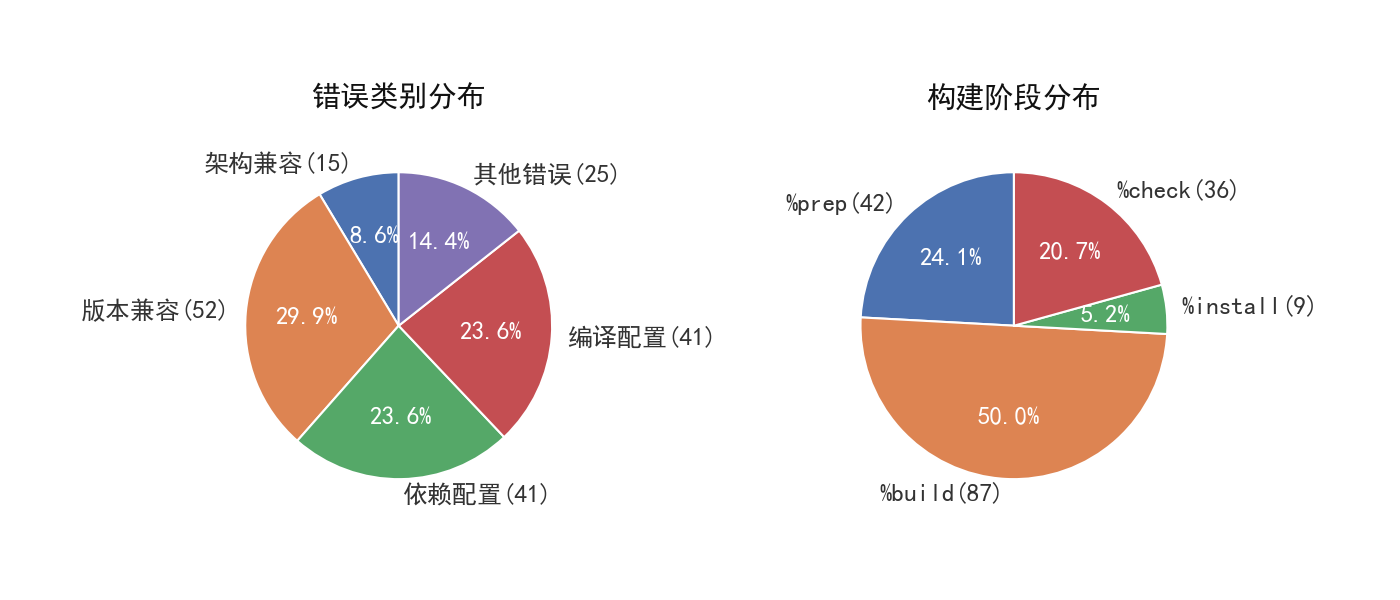
\includegraphics[width=1\linewidth]{pic/dataset-dist.png}
    \caption{RISC\,-V 构建失败数据集错误类别与构建阶段分布}
    \label{fig:dataset}
\end{figure}

\subsubsection{基线方法}
日志压缩实验选取三种基线：（1）LogSage\cite{r9}——面向长日志的 LLM 驱动分析框架；（2）TemplateRAG——模板化解析与检索增强方法；（3）LogPrompt\cite{r10}——通过提示工程增强 LLM 的日志分析能力。

根因分析实验设置四类对比基线：（1）朴素 RAG Agent——基于语义相似度的经典检索增强生成；（2）LogSage\cite{r9}——改进的多路 RAG 检索增强；（3）MCTS——搜索式推理框架；（4）旗舰推理模型（Seed1.8、Kimi K2、DeepSeekV3.2）——以模型能力为主要提升来源的对照。

\subsubsection{评价指标}
日志压缩以行级 Precision/Recall/F1 评估关键证据保留能力。根因分析采用综合得分函数：
\begin{equation}
\text{score}(i) = \frac{s_i + c_i + r_i + f_i}{4}
\end{equation}
其中 $s_i$ 为关键错误语句提取得分，$c_i$ 为错误分类得分，$r_i$ 为根因解释得分，$f_i$ 为修复建议得分。

\subsection{日志压缩实验结果}

\begin{table}[htbp]
\centering
\caption{日志压缩方法准确性对比}
\label{tab:mgsc-results}
\begin{tabular}{lccc}
\hline
\textbf{方法} & \textbf{Prec} & \textbf{Rec} & \textbf{F1} \\
\hline
LogPrompt & 0.260 & 0.300 & 0.334 \\
TemplateRAG & 0.047 & 0.769 & 0.080 \\
LogSage & 0.308 & 0.574 & 0.387 \\
MGSC（本文） & \textbf{0.302} & \textbf{0.668} & \textbf{0.389} \\
\hline
\end{tabular}
\end{table}

如表~\ref{tab:mgsc-results} 所示，MGSC 的 Recall 为 0.668，显著高于 LogSage（0.574），说明显式错误锚点粗筛与基于实体的回溯补全能够更有效地找回长程因果链上的关键线索。同时 MGSC 的 Precision 远高于 TemplateRAG（0.302 vs 0.047），表明在提升覆盖率的同时仍能抑制大量无关噪声。在性能方面，MGSC 在三组日志上的平均输出 token 为 3442/4234/5502，始终处于几千 token 量级，相比 TemplateRAG（38746/49883/55406）小一个数量级，为后续推理预留了充足上下文预算。运行耗时方面，MGSC 在超长日志下相比 LogPrompt 与 TemplateRAG 可实现约 2.3--3.6$\times$ 的加速。

\subsection{MGSC 消融实验}

为验证各模块贡献，对 MGSC 进行消融实验。

\begin{table}[htbp]
\centering
\caption{MGSC 消融实验结果}
\label{tab:mgsc-ablation}
\begin{tabular}{lccc}
\hline
\textbf{配置} & \textbf{Prec} & \textbf{Rec} & \textbf{F1} \\
\hline
MGSC（完整） & 0.302 & 0.668 & 0.389 \\
w/o Anchor Filter & 0.274 & 0.352 & 0.328 \\
w/o Entity Backtracking & 0.292 & 0.584 & 0.372 \\
w/o Semantic Compressor & 0.246 & 0.668 & 0.349 \\
\hline
\end{tabular}
\end{table}

如表~\ref{tab:mgsc-ablation} 所示，去除错误锚点粗筛（w/o Anchor Filter）后 Recall 由 0.668 降至 0.352（$\downarrow$47.3\%），F1 下降 15.7\%，说明显式错误锚点定位对快速锁定异常区域具有决定性作用。去除实体回溯（w/o Entity Backtracking）时 Recall 与 F1 分别下降 12.6\% 和 4.4\%，表明该模块能有效补齐跨距离因果线索。去除语义压缩模型（w/o Semantic Compressor）后 Recall 不变而 Precision 下降 18.5\%，说明轻量语义压缩主要贡献在于提高输出纯度与结构化摘要的稳定性。

\subsection{根因分析实验结果}

\begin{table}[htbp]
\centering
\caption{根因分析综合性能对比}
\label{tab:hrl-results}
\small
\setlength{\tabcolsep}{3pt}
\begin{tabular}{llccccc}
\hline
\textbf{分组} & \textbf{方法} & $s_i$ & $c_i$ & $r_i$ & $f_i$ & \textbf{Score} \\
\hline
\multirow{4}{*}{\rotatebox{90}{DeepSeekV3}}
& RAG & 0.769 & 0.657 & 0.655 & 0.520 & 0.650 \\
& LogSage & 0.870 & 0.754 & 0.692 & 0.524 & 0.710 \\
& MCTS & 0.881 & 0.777 & 0.714 & 0.567 & 0.735 \\
& HRL-RCA & \textbf{0.892} & \textbf{0.798} & \textbf{0.766} & \textbf{0.706} & \textbf{0.790} \\
\hline
\multirow{4}{*}{\rotatebox{90}{GPT-OSS}}
& RAG & 0.743 & 0.625 & 0.693 & 0.613 & 0.669 \\
& LogSage & 0.791 & 0.699 & 0.721 & 0.606 & 0.704 \\
& MCTS & 0.841 & 0.747 & 0.754 & 0.590 & 0.733 \\
& HRL-RCA & \textbf{0.821} & \textbf{0.745} & \textbf{0.760} & \textbf{0.742} & \textbf{0.767} \\
\hline
\multirow{3}{*}{\rotatebox{90}{旗舰模型}}
& Seed 1.8 & 0.814 & 0.665 & 0.755 & 0.635 & 0.717 \\
& Kimi K2 & 0.833 & 0.713 & 0.744 & 0.592 & 0.721 \\
& DSV3.2 & 0.728 & 0.605 & 0.691 & 0.545 & 0.642 \\
\hline
\end{tabular}
\end{table}

如表~\ref{tab:hrl-results} 所示，HRL-RCA 在两种基座下均取得最高综合得分。在 DeepSeekV3 基座下综合得分为 0.790，较最强基线 MCTS（0.735）提升 5.5\%，较朴素 RAG（0.650）提升 21.5\%。

\begin{figure}[htbp]
    \centering
    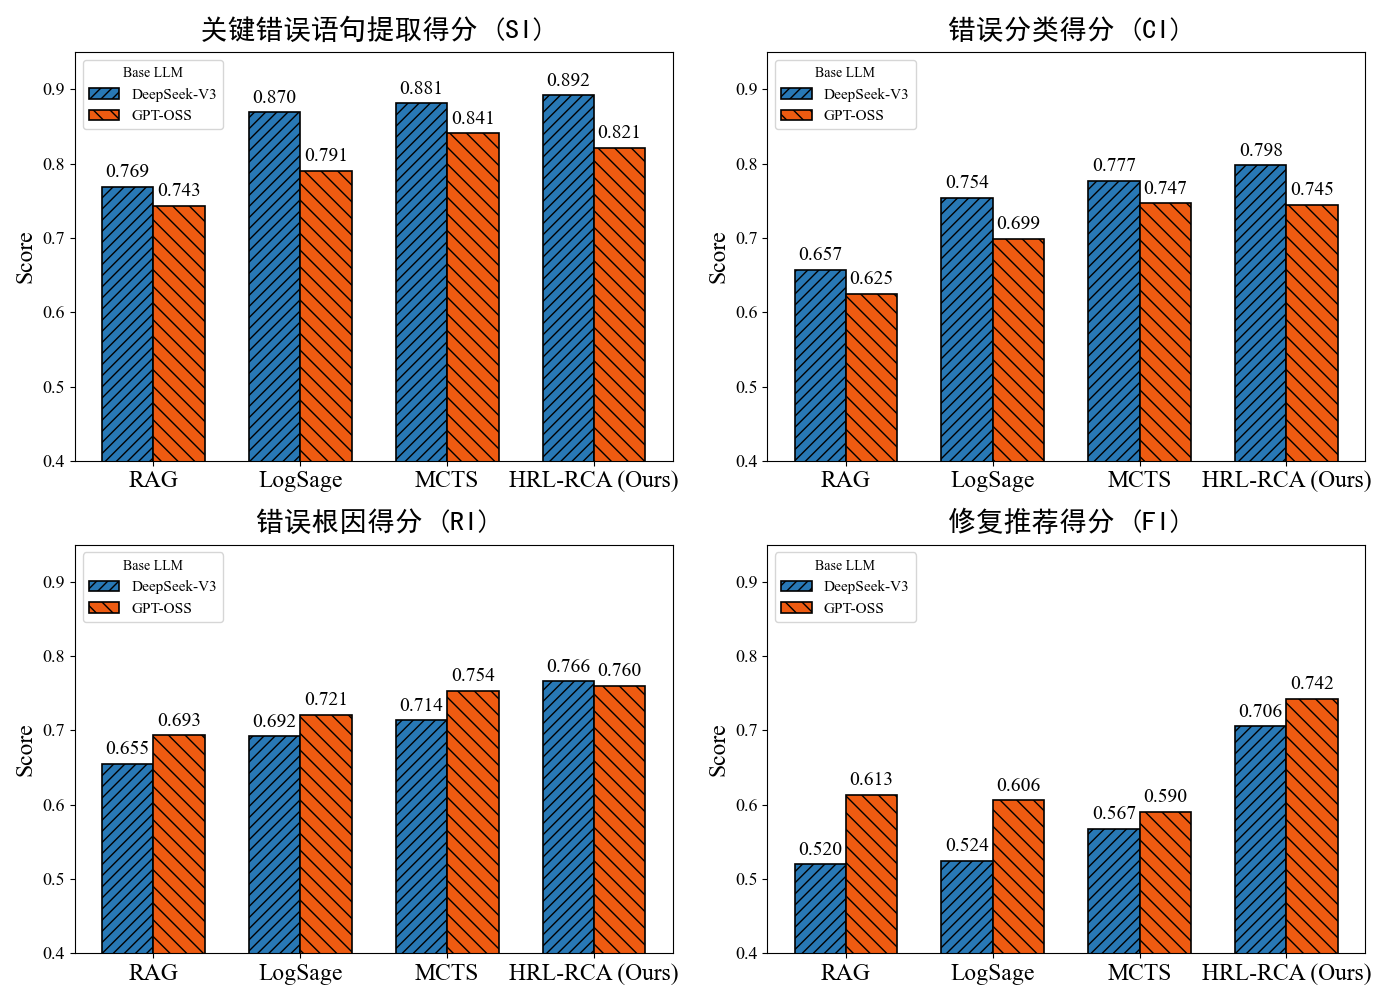
\includegraphics[width=1\linewidth]{pic/4-3-2-1.png}
    \caption{各方法分项得分对比}
    \label{fig:sub-scores}
\end{figure}

如图~\ref{fig:sub-scores} 所示，HRL-RCA 的优势主要体现在修复推荐与根因解释环节：在 DeepSeekV3 基座下修复推荐得分达到 0.706，相比 MCTS 的 0.567 提升 0.139，说明通过历史修复规则的条件路由与证据绑定，更容易在满足适用前提的情况下召回可执行修复依据。关键错误提取得分在各方法中整体较高（0.769--0.892），说明统一的日志语义压缩已提供较强的错误锚点，而 HRL-RCA 仍保持最高（0.892），体现出结构化推理路径对推理稳定性的促进作用。

与独立旗舰推理模型基线相比，Seed1.8、Kimi K2 与 DeepSeekV3.2 的综合得分均低于 HRL-RCA，说明在构建失败这种强依赖适用前提与可验证证据的任务中，仅提升模型推理能力不足以稳定获得高质量修复建议，需要结构化的知识组织与证据约束机制。

\subsection{效率分析}

\begin{figure}[htbp]
    \centering
    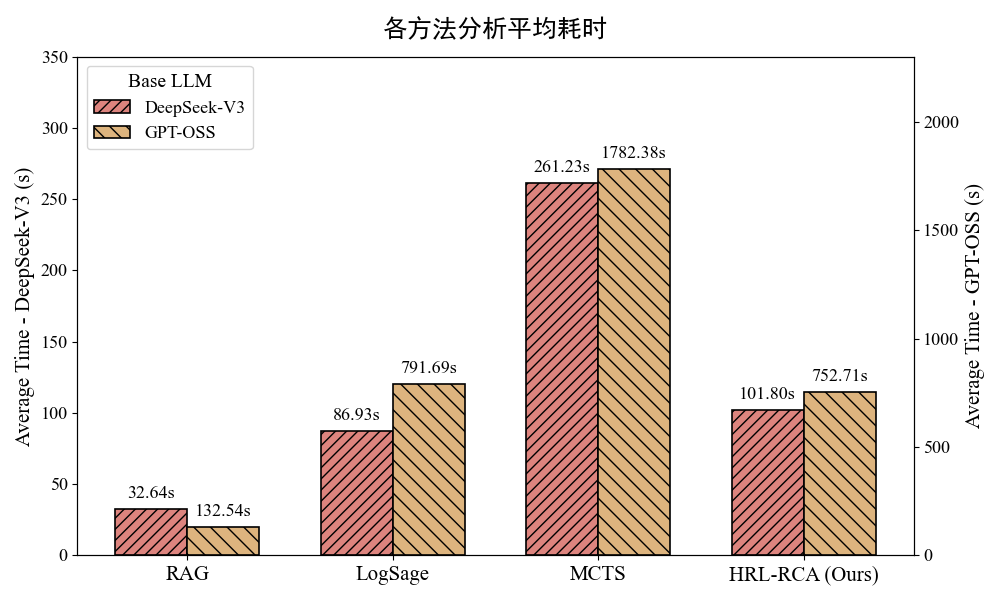
\includegraphics[width=1\linewidth]{pic/4-3-2-2.png}
    \caption{各方法平均处理耗时对比}
    \label{fig:efficiency}
\end{figure}

如图~\ref{fig:efficiency} 所示，HRL-RCA 在 DeepSeekV3 基座下平均耗时 101.80s，相比 MCTS 的 261.23s 减少约 61.0\%，与 LogSage（86.93s）基本持平。朴素 RAG 耗时最短（32.64s），但准确性显著不足。MCTS 因多轮搜索式推理导致耗时最长，而 HRL-RCA 通过规则路由将候选空间限制在局部范围，避免了全局搜索的开销，在保持最优准确性的同时兼顾了工程可用性。


%% ===== 总结与展望 =====
\section{总结与展望}

本文面向 RISC\,-V 软件包构建失败场景，提出"日志压缩 + 规则学习"的两阶段根因分析方法。第一阶段 MGSC 通过显式错误锚点定位、基于实体的跨距离上下文回溯与轻量模型语义压缩，在严格 token 预算下保留高保真证据链，显著降低长日志输入规模。第二阶段 HRL-RCA 将历史修复经验结构化为可判定规则并组织为树形索引，在线推理时通过条件路由召回满足前提的规则，在证据约束下生成可追溯的根因分析与修复建议。

实验结果表明，MGSC 在关键证据覆盖率上优于现有压缩方法，且输出 token 规模稳定可控；HRL-RCA 在综合诊断得分上达到 79.0\%，显著超过朴素 RAG、多路检索增强与搜索式推理等基线，同时处理耗时较 MCTS 降低 61\%，在效率上亦具有明显优势。未来工作将进一步完善规则知识库的增量更新与去重机制，探索将方法适配到更多架构与构建系统，并开发面向开发者的 IDE 插件等工具以促进工程落地。

\vspace{12pt}
\bibliographystyle{IEEEtran}
\bibliography{reference}
\end{document}
